%% Copyright 2018 H.\ Rabus
%
% This work may be distributed and/or modified under the
% conditions of the LaTeX Project Public License, either version 1.3
% of this license or (at your option) any later version.
% The latest version of this license is in
%   http://www.latex-project.org/lppl.txt
% and version 1.3 or later is part of all distributions of LaTeX
% version 2005/12/01 or later.
%
% This work has the LPPL maintenance status `author-maintained'.
%
% This work consists of the file texbsp.tex
%

\documentclass[smallheadings]{scrartcl}

%%% GENERAL PACKAGES %%%%%%%%%%%%%%%%%%%%%%%%%%%%%%%%%%%%%%%%%%%%%%%%%%%%%%%%%%
% inputenc allows the usage of non-ascii characters in the LaTeX source code
\usepackage[utf8]{inputenc}
\usepackage{graphicx} 
\usepackage{float}
%\graphicspath{ {/u/hnatiuka/Praktikum/PPI/} }


% title of the document
\title{Bericht zu Serie 1}
% optional subtitle
%\subtitle{Draft from~\today}
% information about the author
\author{%
  Arsen Hnatiuk,\\%
  Max Huneshagen 
}
\date{\today} 


%%% LANGUAGE %%%%%%%%%%%%%%%%%%%%%%%%%%%%%%%%%%%%%%%%%%%%%%%%%%%%%%%%%%%%%%%%%%
% babel provides hyphenation patterns and translations of keywords like 'table
% of contents'
\usepackage[ngerman]{babel}

%%% HYPERLINKS %%%%%%%%%%%%%%%%%%%%%%%%%%%%%%%%%%%%%%%%%%%%%%%%%%%%%%%%%%%%%%%%
% automatic generation of hyperlinks for references and URIs
\usepackage{hyperref}

%%% MATH %%%%%%%%%%%%%%%%%%%%%%%%%%%%%%%%%%%%%%%%%%%%%%%%%%%%%%%%%%%%%%%%%%%%%%
% amsmath provides commands for type-setting mathematical formulas
\usepackage{amsmath}
% amssymb provides additional symbols
\usepackage{amssymb}
% HINT
% Use http://detexify.kirelabs.org/classify.html to find unknown symbols!

%%% COLORS %%%%%%%%%%%%%%%%%%%%%%%%%%%%%%%%%%%%%%%%%%%%%%%%%%%%%%%%%%%%%%%%%%%%
% define own colors and use colored text
\usepackage[pdftex,svgnames,hyperref]{xcolor}

%%% Code Listings %%%%%%%%%%%%%%%%
% provides commands for including code (python, latex, ...)
\usepackage{listings}
\definecolor{keywords}{RGB}{255,0,90}
\definecolor{comments}{RGB}{0,0,113}
\definecolor{red}{RGB}{160,0,0}
\definecolor{green}{RGB}{0,150,0}
\lstset{language=Python, 
        basicstyle=\ttfamily\small, 
        keywordstyle=\color{keywords},
        commentstyle=\color{comments},
        stringstyle=\color{red},
        showstringspaces=false,
        identifierstyle=\color{green},
        }


\usepackage{paralist}
\usepackage{nicefrac}
% setting the font style for input und returns in description items
\newcommand{\initem}[2]{\item[\hspace{0.5em} {\normalfont\ttfamily{#1}} {\normalfont\itshape{(#2)}}]}
\newcommand{\outitem}[1]{\item[\hspace{0.5em} \normalfont\itshape{(#1)}]}
\newcommand{\bfpara}[1]{
	
	\noindent \textbf{#1:}\,}

\begin{document}

% generating the title page
\maketitle
% generating the table of contents (requires to run pdflatex twice!)
\tableofcontents
\bigskip

\hrule
\hrule

%%% BEGIN OF CONTENT %%%%%%%%%%%%%%%%%%%%%%%%%%%%%%%%%%%%%%%%%%%%%%%%%%%%%%%%%%

\section{Einleitung}
Aus der Theorie der Taylorentwicklung kann man ein günstiges Verfahren zur Approximation der ersten und zweiten Ableitungen einer Funktion ableiten: 
\begin{align}
\label{eq:1_abl}
f'(x)=\underbrace{\frac{f(x+h)-f(x)}{h}}_{:=D_h^{(1)}(x)}+\mathcal{O}(h)
\end{align}
bzw.
\begin{align}
\label{eq:2_abl}
f''(x)=\underbrace{\frac{f(x+h)-2f(x)+f(x-h)}{h^2}}_{:=D_h^{(2)}(x)}+\mathcal{O}(h^2)
\end{align}
mit der Differenziationsschrittweite $h$.

Dieses Verfahren kann sehr nützlich in der numerischen Mathematik sein, jedoch hängt seine Genauigkeit, wie bei jedem Approximationsverfahren, stark von dem Wert der eingegebenen Parameter ab. Deswegen wird eine Studie der Genauigkeit für die sinnvolle Nutzung des Verfahrens benötigt. Die im Teil 1 erstellte Klasse \texttt{Differenzieren} in \texttt{differnzieren.py} erlauben eine numerische Analyse der Beziehung zwischen der Genauigkeit der Approximation und den Parametern. 

\section{Theorie}
Die in der Einleitung genannten Formeln  \eqref{eq:1_abl} und~\eqref{eq:2_abl}  lassen sich aus der Theorie der Taylorentwicklung wie folgt ableiten:
Für eine glatte reellwertige Funktion $f$, für $x\in\mathbb{R}$ und für $h$ in einer passenden Umgebung von $x$ gilt
\begin{align}
f(x+h)&=\sum_{k=0}^{\infty}\frac{f^{(k)}(x)}{k!}h^k\\
&=f(x)+f'(x)h+\sum_{k=2}^{\infty}\frac{f^{(k)}(x)}{k!}h^k
\label{eq:taylor_neg_h}
\end{align}
Das Lösen nach $f'(x)$ liefert:
\begin{align}
f'(x)&=\frac{f(x+h)-f(x)}{h}-\sum_{k=2}^{\infty}\frac{f^{(k)}(x)}{k!}h^{k-1}\\
&=\frac{f(x+h)-f(x)}{h}+\mathcal{O}(h)
\end{align}
Die zweite Formel erhält man auf eine ähnliche Weise. Wir können die Taylorentwicklung auf ein negatives $h$ anwenden:
\begin{align}
f(x-h)&=\sum_{k=0}^{\infty}\frac{f^{(k)}(x)}{k!}(-h)^k\\
&=f(x)-f'(x)h+\frac{f''(x)h^2}{2} +\sum_{k=3}^{\infty}\frac{f^{(k)}(x)}{k!}(-h)^k
\label{eq:taylor_pos_h}
\end{align}
Addition von \eqref{eq:taylor_pos_h} und \eqref{eq:taylor_neg_h} liefert:
\begin{align}
f(x+h)+f(x-h)=2f(x)+f''(x)h^2+\sum_{k=2}^{\infty}\frac{f^{(2k)}(x)}{(2k)!}h^{2k}.
\end{align}
Das Lösen nach $f''(x)$ ergibt:
\begin{align}
f''(x)=\frac{f(x+h)+f(x-h)-2f(x)}{h^2}+\mathcal{O}(h^2).
\end{align}


Ein anderer wichtiger Begriff für die Bearbeitung folgender Experimente ist die Periodizität der Sinus Abbildung und seiner Ableitungen. Zu einem gegebenen $j\in\mathbb{R}$ ist die Periode von $\sin(jx)$ gleich $\frac{2\pi}{j}$. Die Ableitungen von $\sin(jx)$ verhalten sich auf die gleiche Weise.

\section{Experimente}

\paragraph{Experiment 1}
Für die Veranschaulichung der Genauigkeit der Approximation von den Ableitungen bei Schrittweiten $\frac{\pi}{3}$, $\frac{\pi}{4}$, $\frac{\pi}{5}$ und $\frac{\pi}{10}$ wurde ein Programm geschrieben (\texttt{hauptprogramm2.py}), das den Sinus und seine ersten beiden Ableitungen (approximiert und exakt) im Intervall $\left[a,b\right]:=\left[0,\pi\right]$ plottet. Das Ergebnis ist in Abbildung~\ref{im:ablplot} dargestellt.

\paragraph{Experiment 2}
Im zweiten Experiment soll der maximale Fehler der Approximation 
\begin{align}
e_h^{(k)}:=\max\limits_{i=0,\dots,p}\vert f^{(k)}(x_i)-D_h^{(k)}x_i\vert\text{,~~~~~~~~}k=1,2
\end{align}
wiederum für $f(x)=\sin(x)$ in Abhängigkeit der Differenziationsschrittweite $h$ betrachtet werden. Besonderer Fokus soll hierbei auf das Konvergenzverhalten von $e_h^{(k)}$ gelegt werden. Aus \eqref{eq:1_abl} und \eqref{eq:2_abl} ist sofort ersichtlich, dass aus mathematisch naiver Sicht $e_h^{(k)}\sim h^k$ zu erwarten sein wird. 

\paragraph{Experiment 3}
Weiterhin wird das Konvergenzverhalten von $e_h^{(k)}$ für die Funktion $f_j(x)=\sin(jx)$ untersucht und mit dem des Sinus verglichen. In Experiment~3 wird zunächst der Fall $j<1$ betrachtet. Nach der Bemerkung zur Periodizität von $f_j$ in Abschnitt~\ref{sec:Theo} entspricht dies einer Streckung des Sinus entlang der Abszisse.

\paragraph{Experiment 4}
Im letzten Experiment wird analog zu Experiment~3 vorgegangen, allerdings wird nun der Fall $j>1$ untersucht, also der entlang der x-Achse gestauchte Sinus.


\begin{figure}
	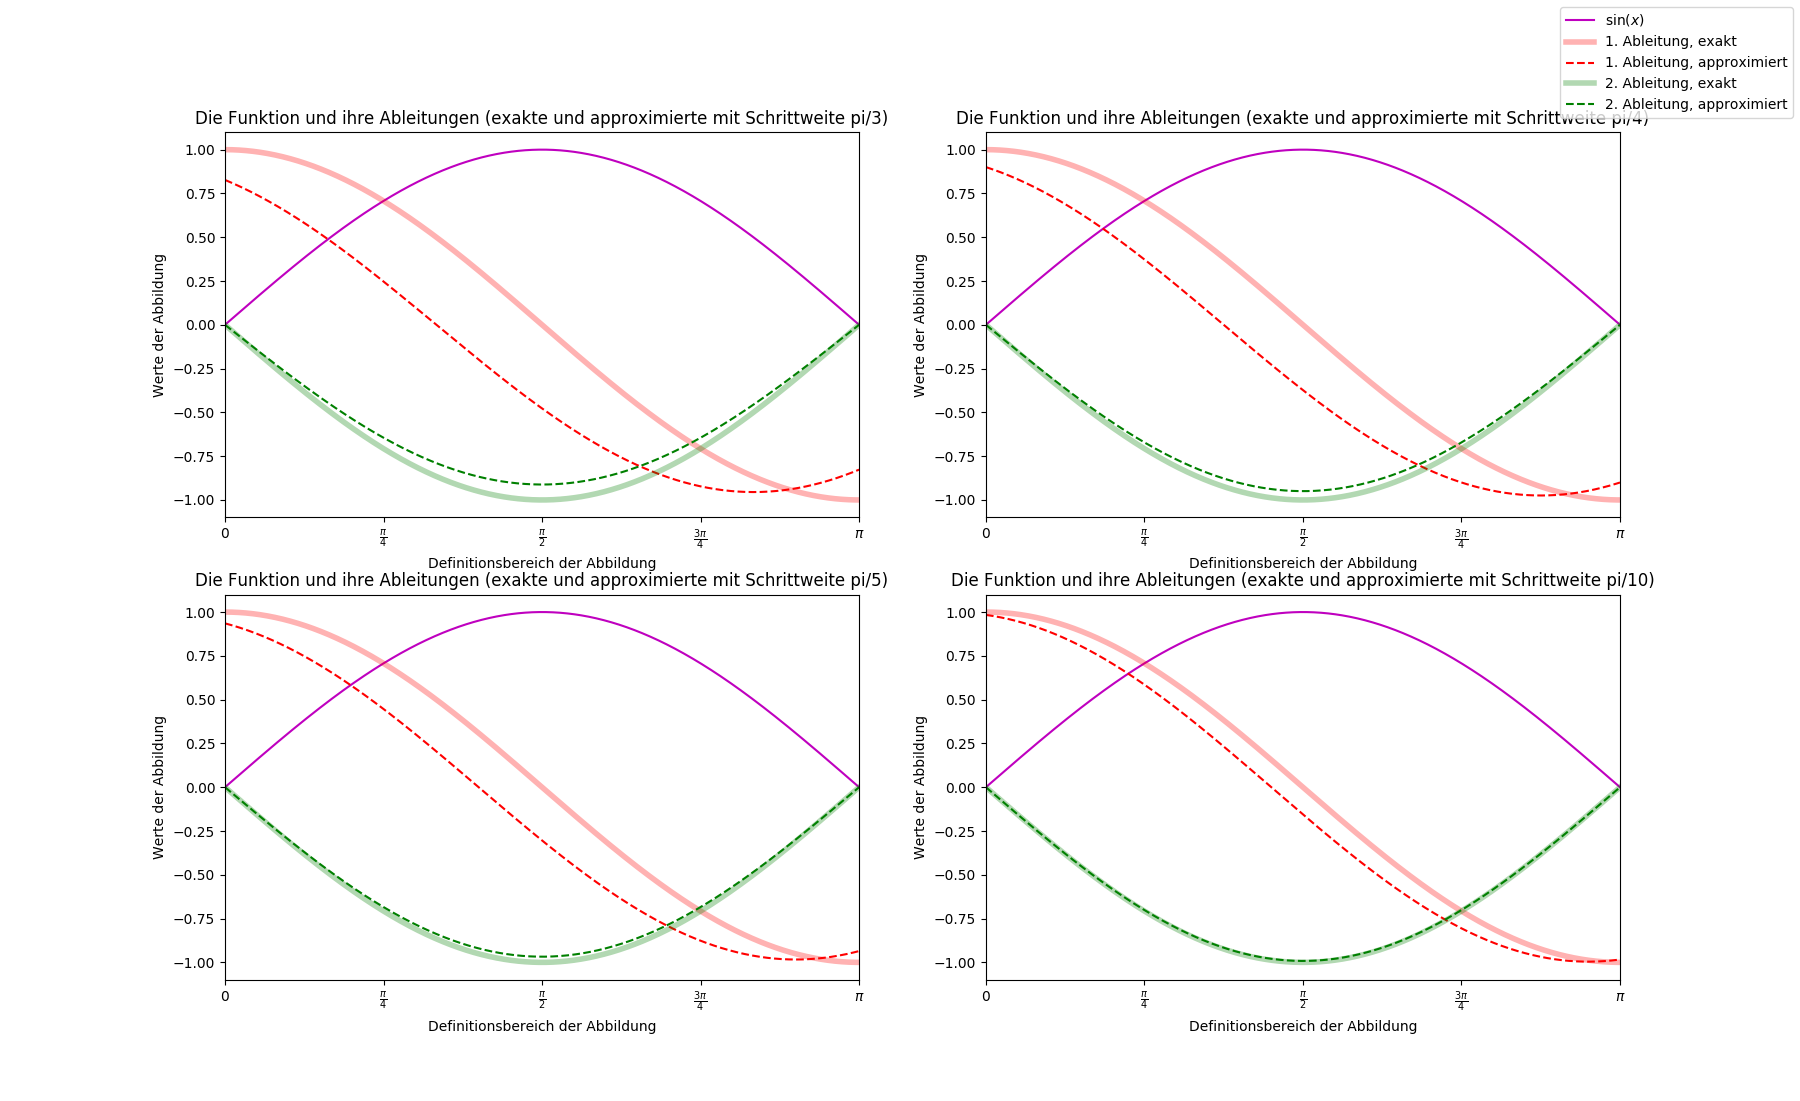
\includegraphics[width=\linewidth]{4Bilder.png}
	\caption{Die approximierten Ableitungen für verschiedene Schrittweiten (Experiment 1).}
	\label{im:ablplot}
\end{figure}

\section{Analyse der Experimente}

\paragraph{Experiment 1}
Aus der graphischen Ausgabe des ersten Experiments in Abb.~\ref{im:ablplot} wird dreierlei ersichtlich; zum Ersten wird die Approximation der beiden Ableitungen mit sinkendem $h$ genauer. Dies stimmt mit der Theorie überein, weil wir erwarten, dass der Fehler in der ersten bzw. zweiten Ableitung der Ordnung $\mathcal{O}(h)$ bzw. $\mathcal{O}(h^2)$ ist. 

Zweitens ist die die Approximation der ersten Ableitung im Vergleich zu den genauen Daten nach Rechts verschoben. Dies ist auch erwartet, der Grund dafür liegt in der Approximationsformel für die erste Ableitung \ref{eq:1_abl}. Man sieht dort, dass die approximierte Tangente nicht um den Punkt $x$ zentriert ist, sondern um den Mittelpunkt zwischen $x+h$ und $x$. Folglich ist die Approximation um $\frac{h}{2}$ nach rechts verschoben. Dies passiert nicht bei der zweiten Ableitung, weil die entsprechende Formel \ref{eq:2_abl} sowohl auf $x+h$, als auch auf $x-h$ beruht. Dieser Effekt wurde bereits in der Schnittstellendokumentation der Funktion \texttt{Differenzieren.ablapprox} besprochen.

Schließlich ist die Approximation der zweiten Ableitung für diese Schrittweiten genauer als die erste. Wie die erste Beobachtung, liegt dies an die Ordnung der entsprechenden Fehler nach \eqref{eq:1_abl} bzw.~\eqref{eq:2_abl}. Für $h=\frac{\pi}{4}$, $\frac{\pi}{5}$ und $\frac{\pi}{10}$ ist $h^2<h$, und folglich soll die Approximation der zweiten Ableitung genauer sein, als die erste. Für $h=\frac{\pi}{3}$ lässt sie die höhere Genauigkeit der zweiten Ableitung durch die oben beschriebene Verschiebung in der ersten Ableitung erklären. 

\paragraph{Experiment 2}
%hier Referenz zu Abbildung 2 zu schreiben


Der Fehlerplot zeigt drei verschiedene Tendenzen im Fehlerverhalten in Abhängigkeit von der Schrittweite $h$. In dem mittleren Bereich der Schrittweite (ungefähr für $h\in\left[10^{-8}, 1\right]$ für die erste Ableitung und $h\in[10^{-3}, 1] $ für die zweite) verhält sich der Fehler genau so, wie es die Approximationsformeln andeuten; er ist linear zu $h$ im Fall der Approximation der ersten Ableitung und quadratisch in $h$ im Fall der Approximation der zweiten Ableitung. 

\begin{figure}[H]
	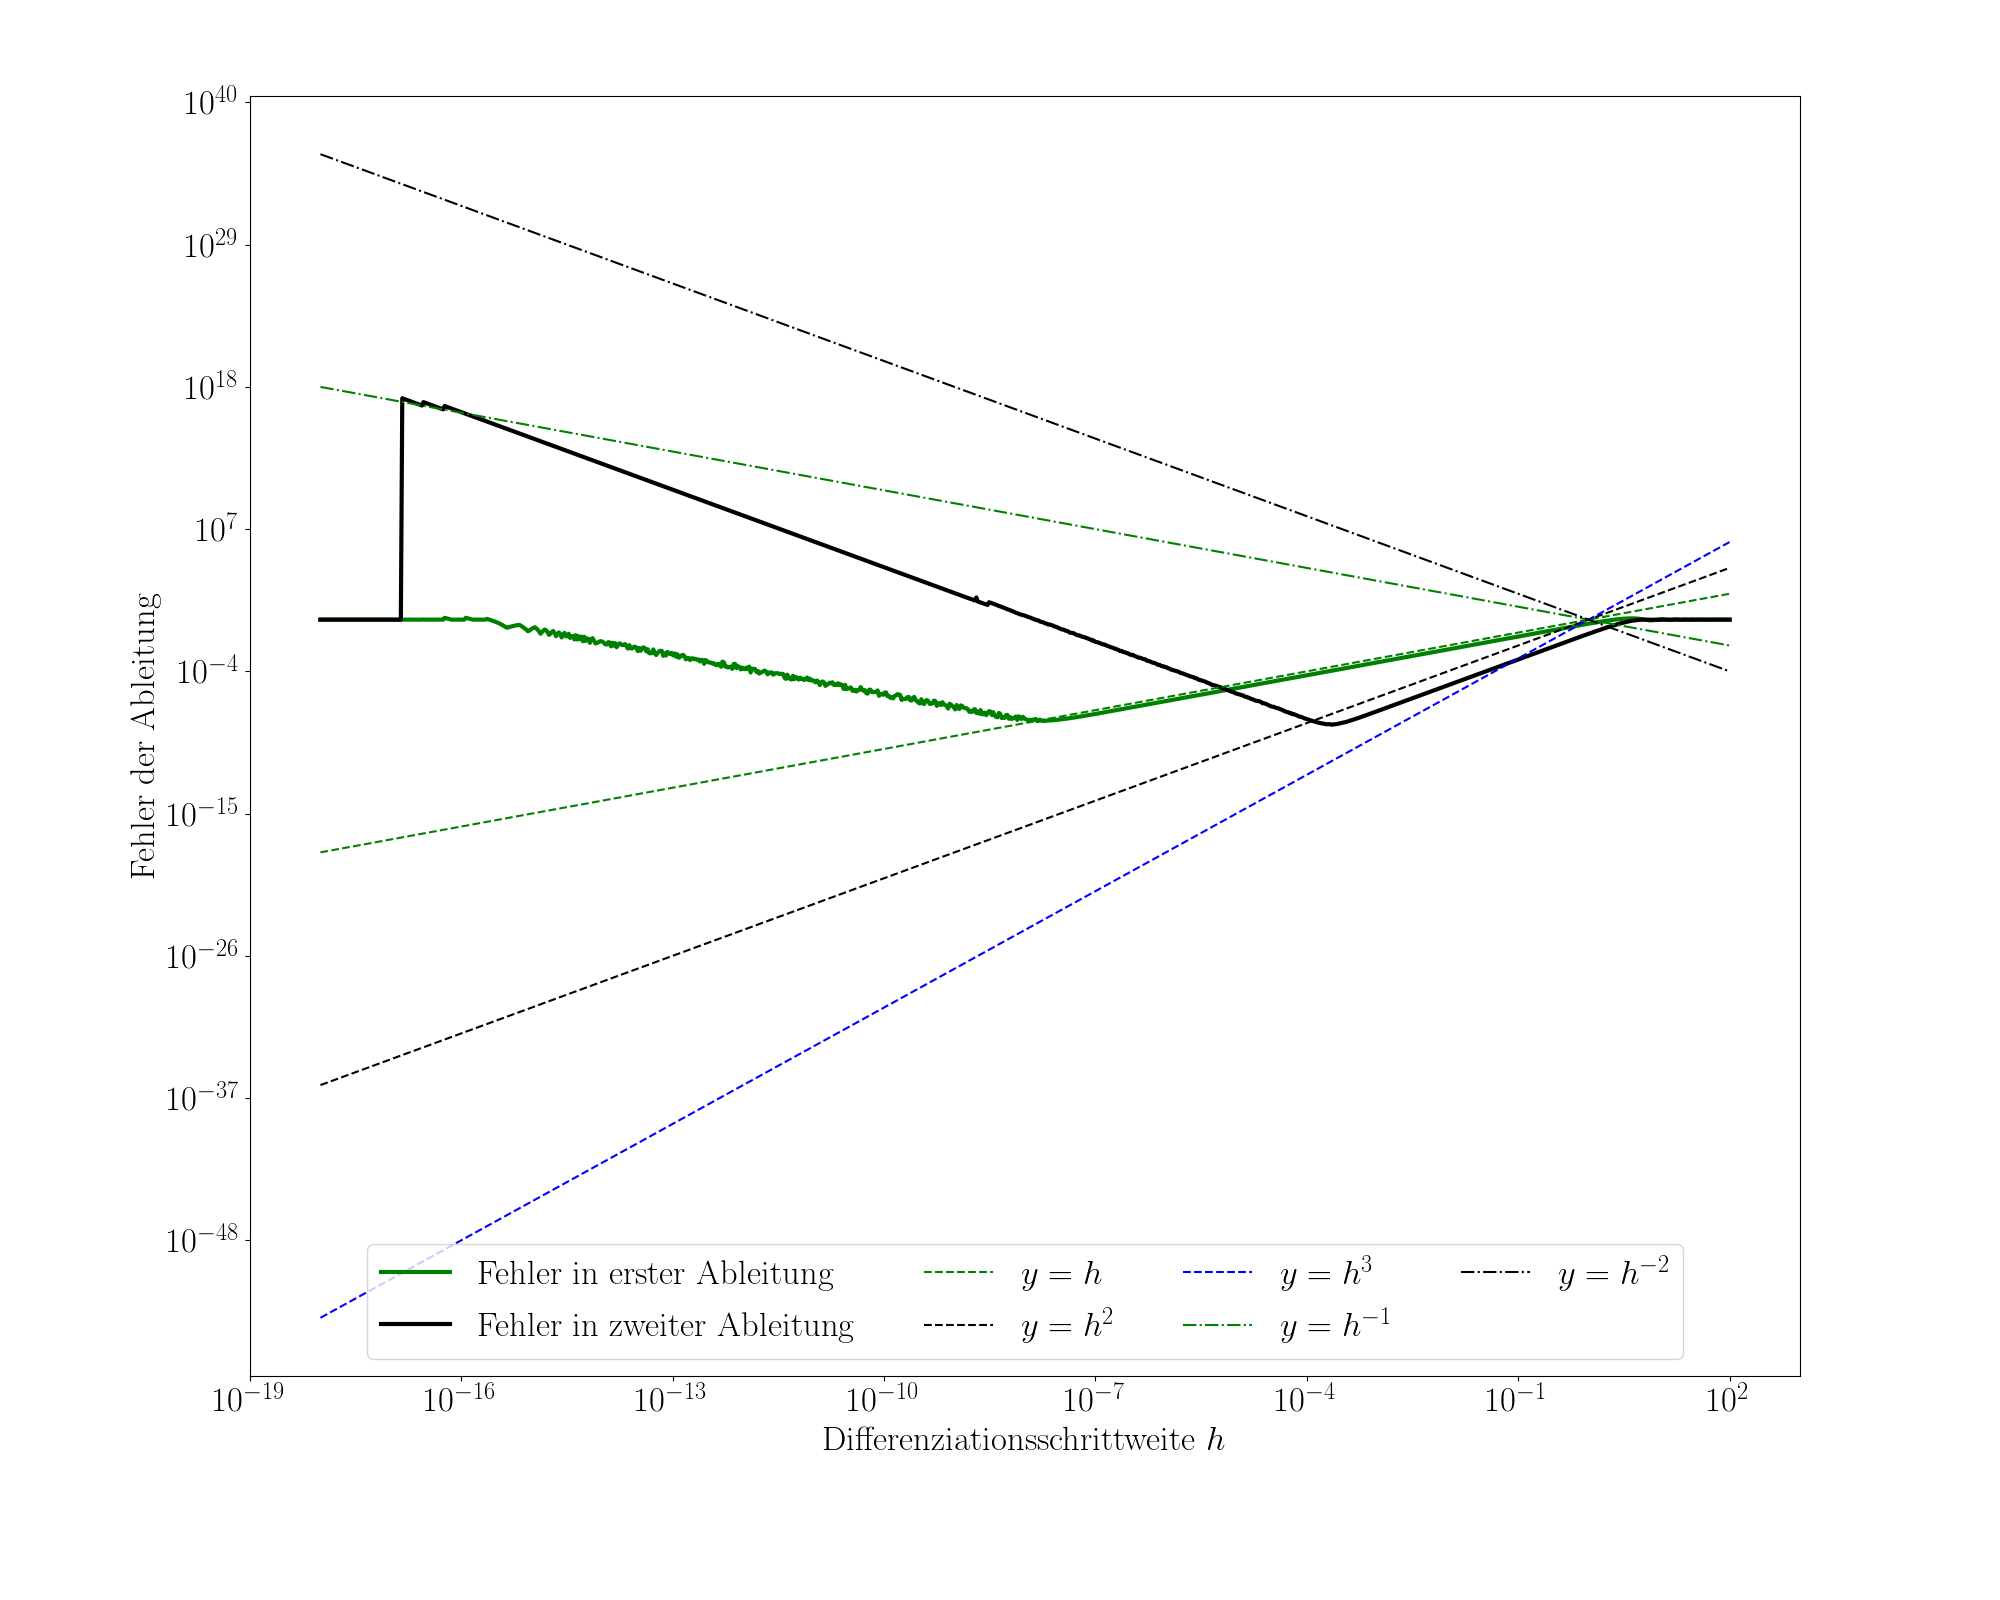
\includegraphics[width=\linewidth]{Bilder/errplot_lang}
	\caption{Maximaler Fehler der beiden ersten Ableitungen des Sinus im Abhängigkeit der Differenziationsschrittweite $h$.}
	\label{im:ablplot}
\end{figure}

Dieses Verhalten ändert sich bei Schrittweiten, die größer als 1 sind. In diesem Bereich konvergiert der Fehler für beide Approximationen gegen 1 für $h\gg1$. Der Grund dafür lässt sich auch aus den Formeln ablesen. Für $f(x)=\sin(x)$ gilt, dass der Zähler des Differenzenquotienten $f(x+h)-f(x)$ betragsmäßig niemals größer als 2 ist. Analog ist der Betrag von $f(x+h)-2f(x)+f(x-h)$ durch 4 beschränkt. Folglich geht bei $h\rightarrow\infty$ der gemäß \eqref{eq:1_abl} bzw.~\eqref{eq:2_abl} approximierte Wert der beiden Ableitungen für alle Punkte $x$ gegen 0. Da diese Werte mit denen der Kosinus bzw. negativen Sinus Abbildungen verglichen werden (diese erreichen im Intervall $\left[0,\pi\right]$ stets den Wert $1$ oder $-1$), konvergiert der maximale Fehler gegen 1. 

Ein anderes Verhalten des Fehlers beobachtet man für sehr kleine Schrittweiten (kleiner als $10^{-8}$ für die erste und $10^{-3}$ für die zweite Ableitung).
In den genannten Bereichen gilt in etwa:
\begin{align}
e_h^{(k)}\sim h^{-k}.
\end{align}
Der Grund hierfür liegt in der finiten Genauigkeit der \texttt{numpy.sin}-Funktion. Während arithmetischer Operationen werden nur 16 Stellen Genauigkeit benutzt\\ (\texttt{numpy.sin(1)-numpy.sin(1+10**-17)}  liefert \texttt{0}). Folglich unterscheiden sich \texttt{numpy.sin(x+h)} und \texttt{numpy.sin(x)} für kleine $h$ in einer Umgebung von $\frac{\pi}{2}$ nur um die allerletzten Nachkommastellen. Also tritt im Ausdruck \texttt{numpy.sin(x+h)-numpy.sin(x)} für genügend kleine Werte von $h$ ein \glqq Rauschen\grqq auf, der Nenner von \eqref{eq:1_abl} bzw.~\eqref{eq:2_abl} wird auch in den vorderen Stellen eine statistisch verteilte Größe. Das gleiche gilt auch für \texttt{sin(x-h)+sin(x+h)-2*sin(h)}. Die approximierte $k$-te Ableitung skaliert nun also mit dem Nenner des Differenzenquotienten: $e_h^{(k)}\sim h^{-k}$. Dieser Verlauf ist in Abb. %TODO Abbildung referenzieren
sichtbar, ebenso wie das rauschen um etwa eine Zehnerpotenz (i.~e.~Rauschen in der ersten Stelle.

Das besagte Rauschen verschwindet wieder für $h\leq 10^{-16}$. Stattdessen liefert $e_h^{(k)}$ den Wert 1 für die erste und zweite Ableitung. %TODO Abbildung hinzufügen
Für beide Ableitungen ist der Fehler in diesem Fall 1. Dies liegt daran, dass \texttt{numpy.sin(x)=numpy.sin(x + 10**-16)}, also sind die approximierten Werte immer 0. Wie im Fall der großen $h$ ist der Fehler dann immer 1.

\begin{figure}[H]
	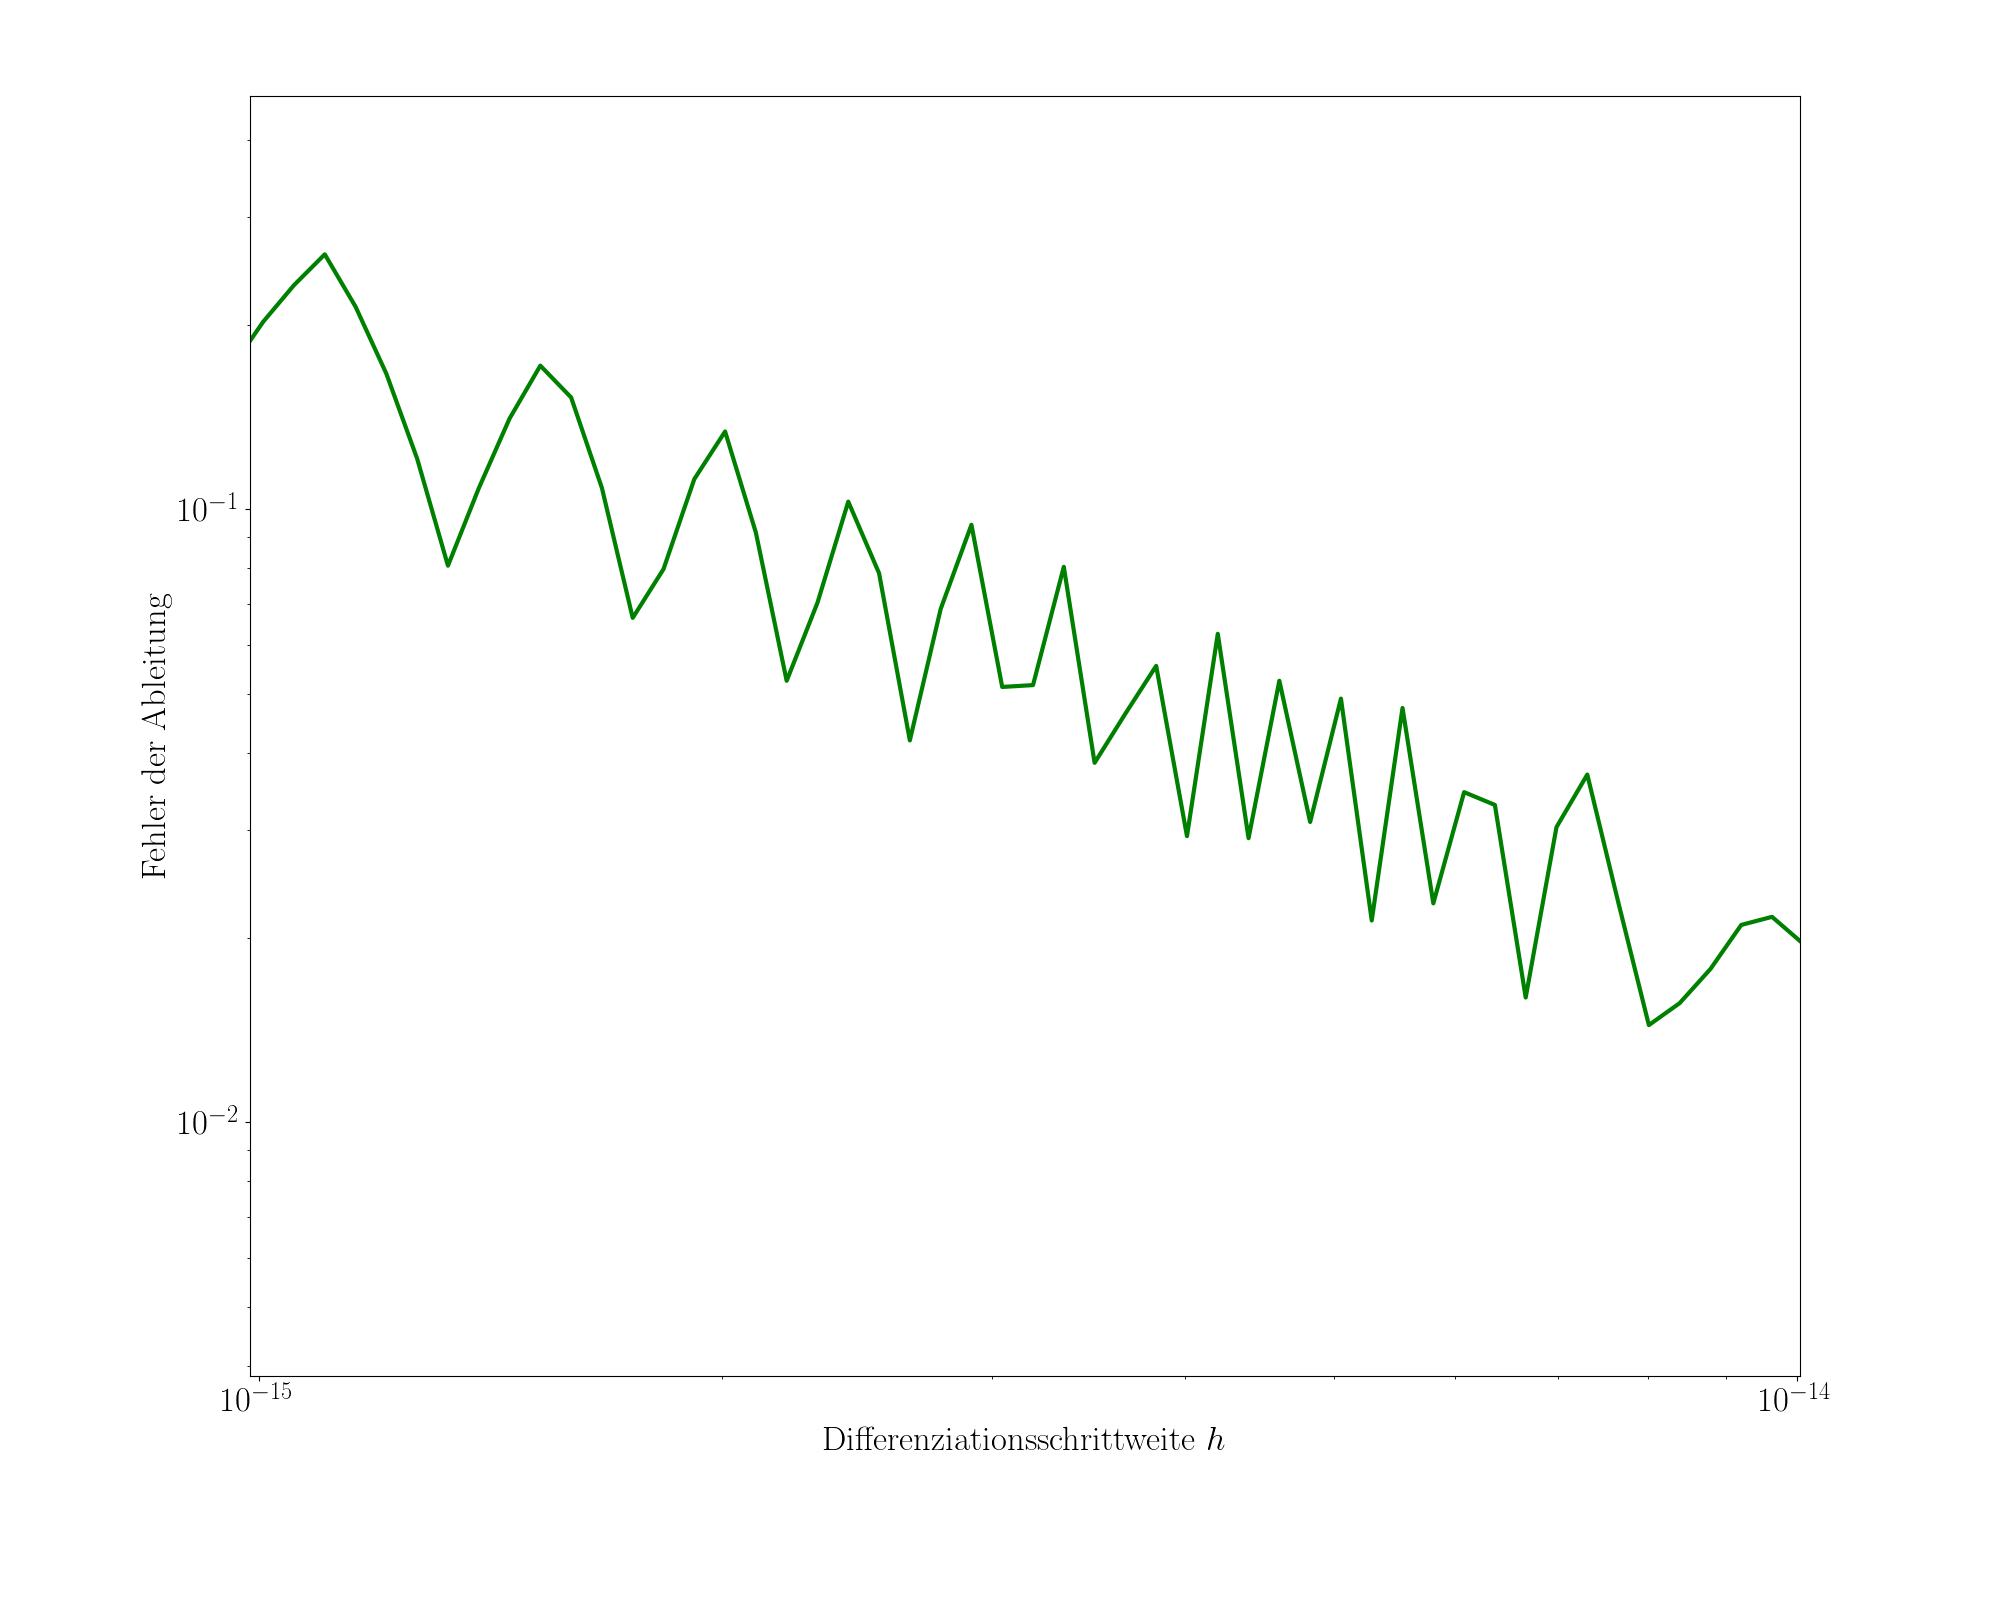
\includegraphics[width=\linewidth]{Bilder/rauschen}
	\caption{Vergrößerte Darstellung des Rauschens in der ersten Ableitung}
	\label{im:rauschen}
\end{figure}

\section{Zusammenfassung}

%%% END OF DOCUMENT %%%%%%%%%%%%%%%%%%%%%%%%%%%%%%%%%%%%%%%%%%%%%%%%%%%%%%%%%%%
\end{document}
